\documentclass[runningheads]{llncs}

\usepackage[T1]{fontenc}
\usepackage[utf8]{inputenc}
\usepackage{graphicx}
\usepackage{xcolor}
\usepackage{amsmath}
\usepackage{booktabs}
\usepackage{longtable}
\usepackage{multirow}
\usepackage{url}
\usepackage[hidelinks]{hyperref}

\renewcommand\UrlFont{\color{blue}\rmfamily}
\graphicspath{{figures/}}

\begin{document}

\title{Beyond the Encounter-Level Benchmark: Patient-Level Validation,
Imbalance Corrections and the Provenance of Signal in 30-Day Hospital
Readmission Prediction}

\titlerunning{Patient-Level Validation of 30-Day Readmission Prediction}

% >>> EDIT THESE THREE LINES BEFORE SUBMITTING <<<
\author{First Last\inst{1}}
\authorrunning{F. Last}
\institute{Your Department, Your Institution, City, Country\\
\email{rkiri98@gmail.com}}

\maketitle

\begin{abstract}
Unplanned readmission within 30 days of discharge is a headline indicator of care
quality and a direct source of financial penalty for hospitals, and the
\emph{Diabetes 130-US Hospitals} database has become the standard public benchmark for
predicting it. Work on that benchmark, however, routinely splits data at the level of
the \emph{encounter} although encounters are nested within patients, applies
resampling to the 11\% minority class almost by reflex, and reports discrimination
without calibration. We conduct an end-to-end investigation on 99{,}340 encounters
from 69{,}987 patients that addresses these three issues directly. Under a strictly
patient-disjoint protocol, a tuned LightGBM model attains AUROC 0.677 (95\% CI
0.668--0.688) and AUPRC 0.223 against a prevalence of 0.113, significantly ahead of
regularised logistic regression ($\Delta$AUPRC $+0.017$, 95\% CI $+0.012$ to
$+0.024$) but far from clinically decisive. Three findings follow. First,
encounter-level splitting shares 36\% of test patients with the training set yet
inflates AUROC by only $0.003$ on average, so the widely repeated leakage concern is
real in principle but immaterial in magnitude for this benchmark --- a negative result
we report explicitly. Second, every imbalance correction we tested failed to improve
ranking while severely degrading calibration: class weighting and undersampling raise
the mean predicted risk from the true 0.113 to 0.46, quadrupling expected calibration
error from 0.003 to above 0.34, and categorical-aware SMOTE-NC \emph{reduces} AUPRC by
30\%. Third, a feature-block ablation shows that demographics alone are
non-informative (AUROC 0.510) and that prior healthcare utilisation supplies almost
all usable signal ($\Delta$AUPRC $-0.047$ when removed), with administrative variables
second. We conclude that the ceiling on this benchmark is a data ceiling rather than a
modelling one, and that the defensible recipe is an uncorrected, well-calibrated
gradient-boosted model evaluated by AUPRC and calibration under patient-level
splitting.

\keywords{Hospital readmission \and Class imbalance \and Calibration \and
Data leakage \and Electronic health records \and Interpretable machine learning}
\end{abstract}

\section{Introduction}

Hospital readmission shortly after discharge is costly, often avoidable, and
increasingly penalised: under the U.S.\ Hospital Readmissions Reduction Program,
hospitals with excess 30-day readmissions lose a share of their Medicare
reimbursement. Diabetes carries a particularly heavy readmission burden, and patients
with diabetes are readmitted at roughly twice the rate of those without. A risk model
that identifies, at the moment of discharge, which patients will bounce back would let
a transitional-care team spend its limited capacity where it matters.

The archetypal public testbed for this problem is the \emph{Diabetes 130-US Hospitals}
database~\cite{strack2014}: ten years of inpatient care, 101{,}766 encounters,
50 variables spanning demographics, diagnoses, laboratory results, medications,
administrative attributes and prior utilisation. It reproduces, in miniature, every
pathology of real hospital records --- extensive and non-random missingness, an
imbalanced outcome, and many interacting variables --- which is precisely what makes
it a useful methodological laboratory.

That very popularity has entrenched three habits that this paper examines. The
database contains 101{,}766 encounters but only 71{,}518 patients, so a random split
places different admissions of the same patient on both sides of the train/test
boundary; the standard remedy is either to discard all but one encounter per patient,
throwing away the prior-utilisation signal, or to ignore the problem. The outcome is
11\% positive, and resampling is applied so routinely that its effect on the
\emph{probabilities} a clinician would act on is rarely checked. And although model
comparisons proliferate, few studies ask which \emph{kinds} of variables --- clinical,
administrative, demographic or historical --- are actually carrying the signal.

\paragraph{Contributions.} We (i) build a reproducible patient-level pipeline with
explicit, informative-missingness-aware feature engineering; (ii) quantify the
optimism created by encounter-level splitting and report the resulting \emph{negative}
finding honestly; (iii) evaluate five treatments of class imbalance on ranking,
calibration and clinical utility simultaneously; (iv) attribute predictive signal to
feature blocks by cumulative and leave-one-out ablation; and (v) release the full
analysis, from literature search log to figures, as executable code.

\section{Related Work}
\label{sec:related}

\subsection{Search protocol}

To avoid a convenience sample of citations, the literature was retrieved
programmatically. Four queries were issued against the OpenAlex API
(Table~\ref{tab:searchlog}) under inclusion criteria fixed \emph{before} searching:
hospitalised adult patients; structured electronic health records; the construct of
readmission risk prediction; machine learning, statistical modelling or feature
engineering on tabular data; published 2015 or later. Exclusion criteria removed
reviews and commentaries without a primary model, studies whose outcome lay outside
the readmission construct, imaging- or genomics-only work, and studies reporting no
predictive performance. Of 100 retrieved records, 77 remained after de-duplication and
23 met all criteria; the decision and reason for every candidate are recorded in
Appendix~\ref{app:screening}. Landmark work falling outside the recency window ---
notably the data statement for the benchmark itself~\cite{strack2014} and the
foundational readmission-model review of Kansagara et al.~\cite{kansagara2011} --- is
cited as background rather than counted as screened evidence.

\begin{table}[htbp]
\centering
\caption{Search log. All queries executed against the OpenAlex API.}
\label{tab:searchlog}
\small
\begin{tabular}{p{1.8cm}p{5.2cm}p{2.1cm}rr}
\toprule
Source & Query & Executed & Hits & Retrieved \\
\midrule
OpenAlex & hospital readmission prediction machine learning EHR & 2026-09-21 08:49 & 6429 & 25 \\
OpenAlex & predicting 30 day readmission missing data class imbalance & 2026-09-21 08:49 & 2625 & 25 \\
OpenAlex & clinical dataset machine learning patient demographics readmission & 2026-09-21 08:49 & 8956 & 25 \\
OpenAlex & electronic health records readmission feature engineering machine learning & 2026-09-21 08:49 & 4325 & 25 \\
\bottomrule
\end{tabular}

\vspace{0.5em}
{\small Retrieved $n=100$; after deduplication $n=77$; screened $n=77$; included $n=23$.}
\end{table}


\subsection{What the literature establishes}

Readmission risk models have a consistent and rather sobering performance ceiling. The
systematic review of Kansagara et al.~\cite{kansagara2011} found that models of the
time discriminated poorly, with c-statistics clustered around 0.60--0.65. Fifteen
years and a methodological generation later, Mahmoudi et al.~\cite{mahmoudi2020},
reviewing 41 EHR-based models in the \emph{BMJ}, reported that richer electronic data
improved on administrative data only modestly, with a median AUROC near 0.68, and that
calibration was rarely reported at all. The scoping review of Huang et
al.~\cite{huang2021scoping} reached the same conclusion for machine learning
specifically: tree ensembles lead, but by margins small enough that dataset and design
choices dominate algorithm choice.

On the benchmark used here, Strack et al.~\cite{strack2014} established the clinical
finding that measuring HbA1c is associated with lower readmission --- a result about
the \emph{ordering of a test}, not about glycaemic control, and one we recover as an
informative-missingness effect in Section~\ref{sec:eda}. Subsequent machine learning
studies on the same data report random forests and boosted ensembles as strongest:
Shang et al.~\cite{shang2021} compared random forests, naive Bayes and decision-tree
ensembles, Lu and Uddin~\cite{lu2022} built an explainable stacking model after random
undersampling, and Liu et al.~\cite{liu2024} compared ten machine learning models with
an LSTM and found random forest and XGBoost ahead of the deep model. All three split
at the encounter level, and none reports calibration.

\subsection{The three gaps}

\paragraph{Patient clustering and leakage.} Kapoor and Narayanan~\cite{kapoor2023}
catalogue data leakage as a leading cause of irreproducible machine-learning claims in
applied science, with non-independence between train and test rows among the most
common forms. Readmission data are a textbook instance: a patient with five admissions
contributes five correlated rows. The size of the resulting optimism on this benchmark
has, to our knowledge, not been measured.

\paragraph{Imbalance corrections.} Resampling is near-universal in this literature ---
Lu and Uddin~\cite{lu2022} undersample, and among the studies we screened the majority
apply SMOTE~\cite{chawla2002} or an undersampling scheme. Yet van den Goorbergh et
al.~\cite{goorbergh2022} show by simulation that imbalance corrections leave
discrimination essentially unchanged while making risk estimates systematically too
high, and Welvaars et al.~\cite{welvaars2023} confirm empirically, on a readmission
case study, that resampling improves apparent performance while producing a gross
overestimation of positive predictions. Because risk models are used to rank and to
\emph{quantify} risk, Van Calster et al.~\cite{vancalster2019} argue that calibration
is the property most often neglected and most consequential. Saito and
Rehmsmeier~\cite{saito2015} add that under imbalance the precision-recall curve is the
informative summary. We test these claims on the benchmark where the opposite practice
prevails.

\paragraph{Provenance of signal.} Model-comparison tables dominate the literature,
while the question of which variable families supply the signal is usually answered,
if at all, by a single feature-importance plot from the winning model. We instead
ablate whole blocks.

\begin{table}[t]
\centering
\small
\caption{Included studies most relevant to this investigation, with the limitation each leaves open.}\label{tab:related}
\begin{tabular}{p{1.7cm}p{2.7cm}p{3.5cm}p{4.0cm}}
\hline\noalign{\smallskip}
Study & Data & Method & Limitation relevant to this work \\
\noalign{\smallskip}\hline\noalign{\smallskip}
\cite{strack2014} & Diabetes 130-US (101,766 enc.) & Multivariable logistic regression & Dataset provenance; one encounter per patient retained, no ML comparison \\
\cite{shang2021} & Diabetes 130-US & Random forest, naive Bayes, decision-tree ensemble & Encounter-level split; accuracy-oriented metrics; calibration not reported \\
\cite{lu2022} & Diabetes 130-US & Stacking ensemble + random undersampling & Undersampling applied before splitting the data; calibration not reported \\
\cite{liu2024} & Diabetes 130-US & 10 ML models + LSTM & Patient clustering not addressed; AUROC-centred comparison \\
\cite{welvaars2023} & Urology readmissions & 7 resampling ratios $\times$ several classifiers & Shows resampling inflates positive predictions; single-centre \\
\cite{goorbergh2022} & Simulation + clinical data & Logistic regression under imbalance corrections & Simulation-based; tree ensembles not examined \\
\cite{amritphale2021} & Nationwide Readmission Database & LR, SVM, DNN, RF, decision tree & Administrative claims only; no laboratory variables \\
\cite{darabi2021} & Stroke EHR ($n=3{,}184$) & RF, GBM, XGBoost, SVM, LR + adaptive sampling & Small cohort; resampling chosen on validation performance \\
\cite{mahmoudi2020} & 41 studies (systematic review) & Narrative synthesis & Reports median AUROC $\approx$ 0.68; few studies report calibration \\
\noalign{\smallskip}\hline
\end{tabular}
\end{table}


\section{Research Problem and Objectives}

\paragraph{Problem statement.} Given the structured record of an inpatient encounter
as it stands at discharge --- demographics, diagnoses, laboratory measurements,
procedures, medications, administrative attributes and the patient's prior utilisation
--- estimate the probability that the patient is readmitted within 30 days, under a
validation protocol that respects the nesting of encounters within patients, and
report that estimate in a form a clinician could act on.

\noindent Formally, for encounter $i$ of patient $g(i)$ with feature vector
$x_i \in \mathcal{X}$ and label $y_i = 1$ if readmitted within 30 days, we seek
$\hat{f}: \mathcal{X} \to [0,1]$ approximating $P(y=1 \mid x)$, evaluated on a test set
whose patients satisfy $g(i) \notin \mathcal{G}_{\text{train}}$.

\paragraph{Objectives and research questions.}
\begin{description}
  \item[O1] Construct a reproducible, leakage-free pipeline with principled handling
    of non-random missingness and domain-driven feature engineering.
  \item[RQ1] How do regularised logistic regression, random forests and gradient
    boosting compare under an identical patient-level protocol, and is any difference
    clinically meaningful?
  \item[RQ2] How much optimism does encounter-level splitting introduce?
  \item[RQ3] Do imbalance corrections improve discrimination, calibration or clinical
    utility?
  \item[RQ4] Which feature blocks carry the predictive signal, and which individual
    predictors drive risk?
\end{description}

\section{Data and Methods}

\subsection{Dataset and justification}

We use the \emph{Diabetes 130-US Hospitals for Years 1999--2008} database from the UCI
Machine Learning Repository (ID 296), donated by Strack et al.~\cite{strack2014} under
a CC BY 4.0 licence: 101{,}766 de-identified inpatient encounters of patients with
diabetes from 130 US hospitals over ten years, described by 49 predictors and a
three-level readmission label.

The choice is deliberate rather than conventional. The dataset is the only large
public inpatient resource that simultaneously carries all six variable families named
in the problem statement \emph{and} an explicit 30-day readmission label; richer
alternatives such as MIMIC-IV are ICU-centric and require credentialed access. It
retains a pseudonymous patient identifier, without which RQ2 could not be posed at
all. Its extensive use makes our numbers directly comparable with published
work~\cite{shang2021,lu2022,liu2024}. And it exhibits, unusually honestly, the
pathologies the problem statement highlights: missingness up to 96.9\%, an 1:7.8 class
imbalance, and strongly interacting variables.

\subsection{Cohort construction}

Encounters ending in death or discharge to hospice ($n=2{,}423$) cannot by
construction be followed by a readmission and are removed, as are three encounters
with invalid gender, leaving \textbf{99{,}340 encounters from 69{,}987 patients}.
Unlike much prior work we retain \emph{all} encounters of a patient rather than only
the first: discarding repeat admissions would destroy the prior-utilisation signal
that Section~\ref{sec:ablation} shows to be dominant. The resulting dependence is
handled at the splitting stage instead. The target is binary, $y=1$ for
\texttt{readmitted} $=$ ``$<$30'', giving a prevalence of \textbf{11.39\%}
(11{,}314 positive encounters).

\subsection{Missing data}

Missingness is extensive and, critically, not ignorable (Table~\ref{tab:missing}). We
test each variable's missingness indicator against the outcome with a $\chi^2$ test.
\texttt{weight} is missing for 96.9\% of encounters with no association to the outcome
($p=1.00$) and is dropped. In contrast \texttt{A1Cresult} is missing for 83.1\% of
encounters precisely when the test was \emph{not ordered}, and that fact is strongly
associated with readmission ($p<10^{-10}$); \texttt{max\_glu\_serum},
\texttt{medical\_specialty}, \texttt{payer\_code} and \texttt{race} behave likewise.
Imputing such values would erase a real signal --- the clinician's decision to
investigate. We therefore encode ``Not measured''/``Missing'' as an explicit level and
add binary \emph{testing} indicators, a choice that follows directly from the test
rather than from convention.

\begin{table}[t]
\centering
\small
\caption{Missing data and the informativeness of missingness. $p$-values are from $\chi^2$ tests of the missingness indicator against the outcome.}\label{tab:missing}
\resizebox{\textwidth}{!}{\begin{tabular}{lrrrr}
\hline\noalign{\smallskip}
Variable & Missing (\%) & Readm. if missing (\%) & Readm. if observed (\%) & $p$ \\
\noalign{\smallskip}\hline\noalign{\smallskip}
weight & 96.9 & 11.4 & 11.4 & 1.000 \\
max\_glu\_serum & 94.8 & 11.3 & 12.8 & 0.002 \\
A1Cresult & 83.1 & 11.7 & 9.9 & $<$0.001 \\
medical\_specialty & 48.9 & 11.8 & 11.0 & $<$0.001 \\
payer\_code & 39.7 & 11.7 & 11.2 & 0.016 \\
race & 2.2 & 8.4 & 11.5 & $<$0.001 \\
diag\_3 & 1.4 & 6.4 & 11.5 & $<$0.001 \\
diag\_2 & 0.4 & 8.1 & 11.4 & 0.065 \\
diag\_1 & 0.0 & 25.0 & 11.4 & 0.118 \\
\noalign{\smallskip}\hline
\end{tabular}}
\end{table}


\subsection{Feature engineering}

Thirty-four predictors (19 numeric, 15 categorical; 123 columns after one-hot
encoding) were derived and grouped into five blocks used throughout the ablation:

\begin{itemize}\setlength\itemsep{1pt}
  \item \textbf{Demographic}: age band mapped to its midpoint, race (with an explicit
    \texttt{Missing} level), gender.
  \item \textbf{Administrative (non-clinical)}: admission type, admission source and
    discharge disposition collapsed into clinically coherent groups; payer code;
    medical specialty (15 most frequent, else \texttt{Other}/\texttt{Missing}).
  \item \textbf{Clinical}: the three ICD-9 diagnosis fields mapped to nine diagnostic
    chapters following~\cite{strack2014}; number of diagnoses; HbA1c and glucose
    results plus their testing indicators; length of stay; counts of laboratory
    procedures, procedures and medications; laboratory tests and medications per day.
  \item \textbf{Medication}: number of active diabetes drugs and number of dose changes
    across the 23 drug variables, insulin regimen, \texttt{change},
    \texttt{diabetesMed}.
  \item \textbf{Prior utilisation}: outpatient, emergency and inpatient visits in the
    preceding year, their sum, binary indicators for any prior inpatient or emergency
    contact, and the index of the encounter within the patient's own history.
\end{itemize}

\subsection{Validation protocol}

The train/test split is a 75/25 \texttt{GroupShuffleSplit} on \texttt{patient\_nbr}
(74{,}583 encounters from 52{,}490 patients versus 24{,}757 from 17{,}497; zero
patient overlap), and hyperparameters are selected by 3-fold
\texttt{StratifiedGroupKFold} randomised search on the training patients only,
optimising average precision. Four families are tuned under an identical budget:
$L_1/L_2$-regularised logistic regression, random forest~\cite{breiman2001},
XGBoost~\cite{chen2016} and LightGBM~\cite{ke2017}, all via
scikit-learn~\cite{pedregosa2011}. A constant model predicting the training prevalence
is the no-skill reference. For RQ2 the entire protocol is repeated with a stratified
random split of encounters, holding model configurations fixed.

\subsection{Evaluation}

Given 11\% prevalence, accuracy is uninformative. We report AUROC; AUPRC, whose
no-skill value is the prevalence~\cite{saito2015}; the Brier score and 10-bin expected
calibration error (ECE); sensitivity, PPV and number-needed-to-evaluate at a
\textbf{10\% alert rate}, the realistic constraint in which a transitional-care team
can follow up the top risk decile; and net benefit by decision-curve
analysis~\cite{vickers2006}. Confidence intervals are bootstrap percentiles over 400
resamples, and model differences are tested by paired bootstrap over 800 resamples.
Reporting follows the spirit of TRIPOD~\cite{collins2015}.

\section{Exploratory Analysis}
\label{sec:eda}

\begin{figure}[t]
\centering
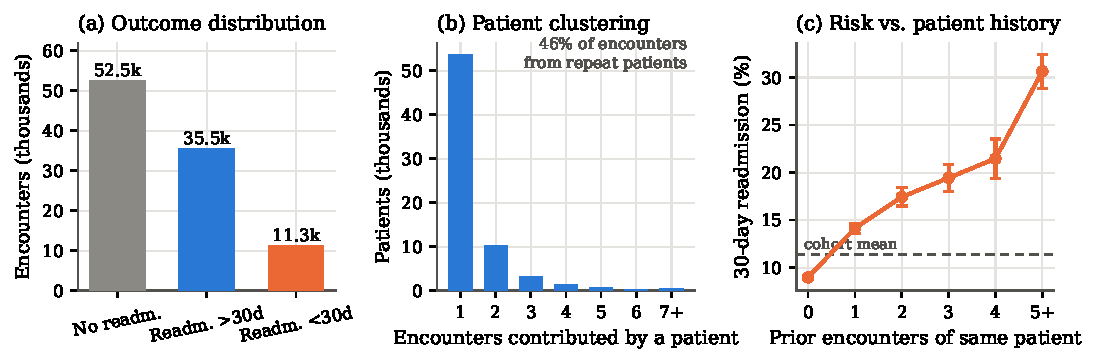
\includegraphics[width=\textwidth]{fig_outcome.pdf}
\caption{(a) Outcome distribution: 11.4\% of encounters are followed by readmission
within 30 days. (b) Patients contribute up to 40 encounters; 46.0\% of encounters come
from patients seen more than once. (c) Readmission risk rises monotonically with the
number of prior encounters the same patient contributes, from 8.98\% to 30.65\% ---
the mechanism that makes both patient-level splitting and prior-utilisation features
consequential. Error bars are 95\% Wald intervals.}
\label{fig:outcome}
\end{figure}

Figure~\ref{fig:outcome} summarises the outcome and the patient clustering that
motivates RQ2. Of 34 engineered predictors, 30 show a statistically significant
univariate association with the outcome after Bonferroni correction --- an expected
consequence of $n\approx10^5$, and the reason we rank by effect size rather than by
$p$-value (Fig.~\ref{fig:assoc}). The ordering is unambiguous: the five strongest
associations are all prior-utilisation variables, led by the number of prior inpatient
visits (rank-biserial $r=0.21$), ahead of every clinical and demographic variable.

\begin{figure}[t]
\centering
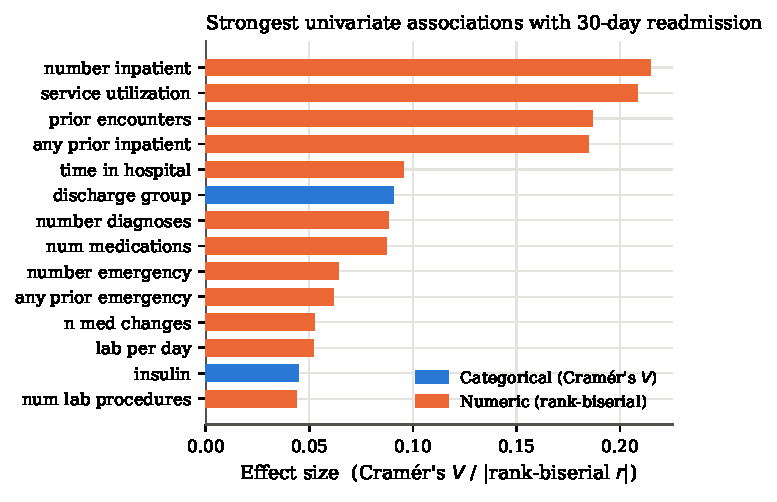
\includegraphics[width=0.72\textwidth]{fig_assoc.pdf}
\caption{Univariate effect sizes. Prior-utilisation variables dominate; age, the
canonical demographic risk factor, ranks fifteenth.}
\label{fig:assoc}
\end{figure}

\begin{figure}[t]
\centering
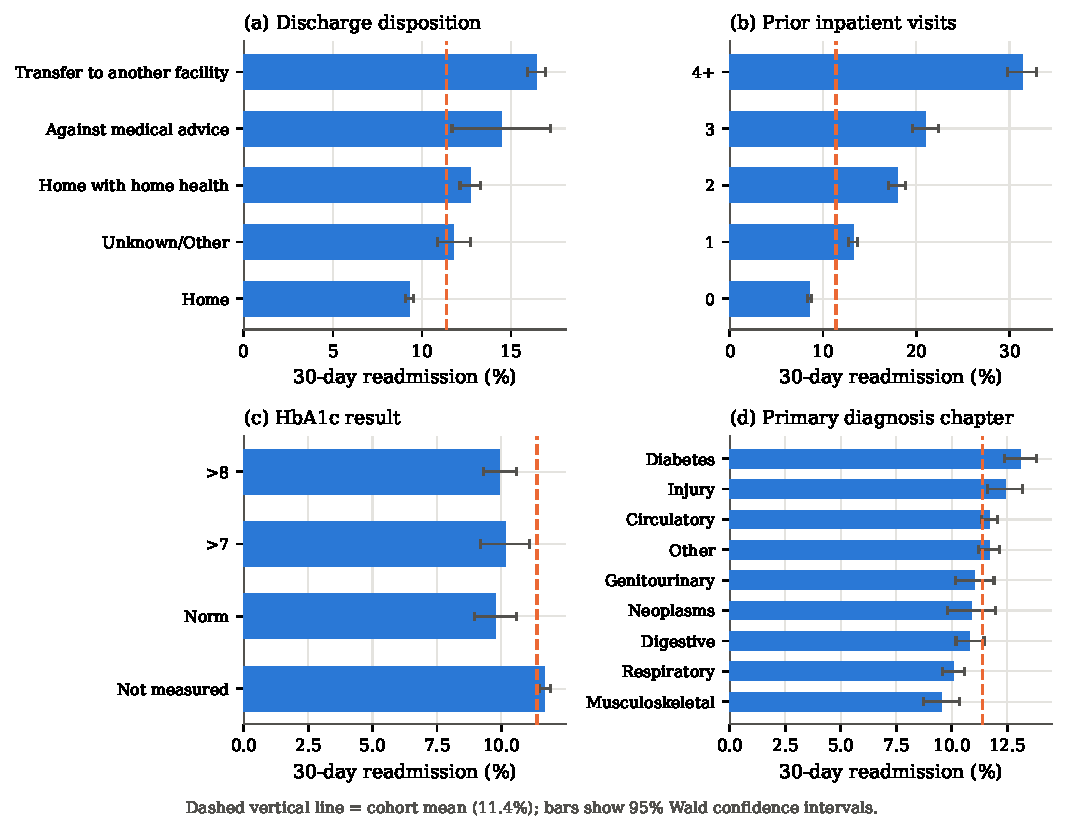
\includegraphics[width=\textwidth]{fig_riskstrat.pdf}
\caption{Readmission rate by candidate predictor, with 95\% Wald intervals; the dashed
line is the cohort mean. Transfer to another facility, prior inpatient visits, an
unmeasured HbA1c and a primary diagnosis of diabetes all mark elevated risk.}
\label{fig:riskstrat}
\end{figure}

Figure~\ref{fig:riskstrat} stratifies risk. Patients with four or more prior inpatient
visits are readmitted at 31.4\% versus 8.6\% for those with none --- a 3.7-fold
gradient that no clinical variable in the dataset approaches. Discharge to another
facility carries 16.4\% risk against 9.2\% for discharge home. Panel (c) reproduces
the effect reported by Strack et al.~\cite{strack2014} in our cohort: encounters in
which HbA1c was \emph{not measured} are readmitted at 11.7\% against 9.8\% when the
result was normal. The clinically important reading is that this is a property of the
care process, not of the patient's glycaemia. Table~\ref{tab:cohort} gives the full
cohort comparison.

\begin{table}[t]
\centering
\small
\caption{Cohort characteristics by 30-day readmission status.}\label{tab:cohort}
\resizebox{\textwidth}{!}{\begin{tabular}{lccc}
\hline\noalign{\smallskip}
Characteristic & Not readmitted $<$30 d & Readmitted $<$30 d & $p$ \\
\noalign{\smallskip}\hline\noalign{\smallskip}
Age (years, median [IQR]) & 65 [55--75] & 65 [55--75] & $<$0.001 \\
Length of stay (days) & 4 [2--6] & 4 [2--6] & $<$0.001 \\
Laboratory procedures & 44 [31--57] & 45 [33--58] & $<$0.001 \\
Medications administered & 15 [10--20] & 16 [11--21] & $<$0.001 \\
Diagnoses recorded & 8 [6--9] & 9 [6--9] & $<$0.001 \\
Prior inpatient visits & 0 [0--1] & 0 [0--2] & $<$0.001 \\
Prior emergency visits & 0 [0--0] & 0 [0--0] & $<$0.001 \\
Prior outpatient visits & 0 [0--0] & 0 [0--0] & $<$0.001 \\
Female & 53.8\% & 54.2\% & 0.428 \\
Race recorded as Caucasian & 74.6\% & 75.6\% & 0.019 \\
Race missing & 2.3\% & 1.7\% & $<$0.001 \\
Discharged home & 62.1\% & 49.5\% & $<$0.001 \\
Transferred to another facility & 19.7\% & 30.2\% & $<$0.001 \\
HbA1c not measured & 82.8\% & 85.2\% & $<$0.001 \\
Primary diagnosis: circulatory & 29.8\% & 30.7\% & 0.054 \\
Primary diagnosis: diabetes & 8.5\% & 10.0\% & $<$0.001 \\
On diabetes medication & 76.8\% & 80.3\% & $<$0.001 \\
Any medication dose change & 46.1\% & 49.0\% & $<$0.001 \\
\noalign{\smallskip}\hline
\end{tabular}
\\[2pt] {\footnotesize $n=88,026$ versus $n=11,314$ encounters. Continuous variables: Mann--Whitney $U$; categorical: $\chi^2$.}}
\\[3pt]
\begin{minipage}{\textwidth}\centering {\footnotesize $n=88,026$ versus $n=11,314$ encounters. Continuous variables: Mann--Whitney $U$; categorical: $\chi^2$.}\end{minipage}
\end{table}


\section{Results}

\subsection{RQ1: model comparison}

\begin{table}[t]
\centering
\small
\caption{Held-out performance on the patient-disjoint test set. Bracketed values are bootstrap 95\% confidence intervals over 400 resamples.}\label{tab:results}
\resizebox{\textwidth}{!}{\begin{tabular}{lcccccc}
\hline\noalign{\smallskip}
Model & AUROC [95\% CI] & AUPRC [95\% CI] & Brier & ECE & Sens@10\% & PPV@10\% \\
\noalign{\smallskip}\hline\noalign{\smallskip}
Baseline (prevalence) & 0.500 [0.500, 0.500] & 0.113 [0.109, 0.117] & 0.100 & 0.002 & 8.7 & 9.9 \\
Logistic regression & 0.664 [0.654, 0.675] & 0.206 [0.194, 0.220] & 0.227 & 0.355 & 21.2 & 23.9 \\
Random forest & 0.674 [0.665, 0.685] & 0.219 [0.206, 0.235] & 0.203 & 0.319 & 22.7 & 25.6 \\
XGBoost & 0.675 [0.666, 0.686] & 0.217 [0.204, 0.232] & 0.223 & 0.350 & 22.7 & 25.6 \\
LightGBM & 0.677 [0.668, 0.688] & 0.223 [0.209, 0.238] & 0.220 & 0.343 & 23.5 & 26.5 \\
\noalign{\smallskip}\hline
\end{tabular}
}
\\[3pt]
\begin{minipage}{\textwidth}\centering {\footnotesize Patient-disjoint test set ($n=24757$ encounters, prevalence 11.3\%). All models except the baseline carry an in-learner imbalance correction; Sens@10\% and PPV@10\% are computed at the threshold that flags the highest-risk decile.}\end{minipage}
\end{table}


\begin{figure}[t]
\centering
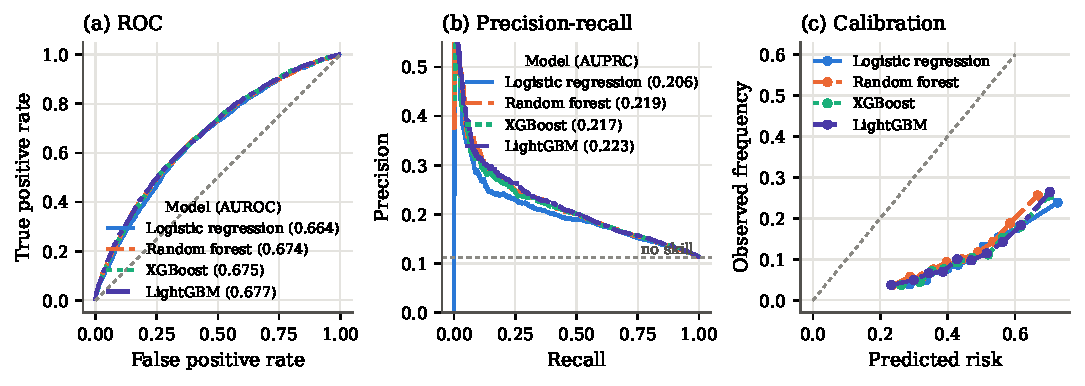
\includegraphics[width=\textwidth]{fig_performance.pdf}
\caption{Held-out performance on the patient-disjoint test set. Discrimination is
modest and nearly identical across families; panel (c) exposes the calibration failure
induced by the in-learner imbalance corrections these models carry.}
\label{fig:performance}
\end{figure}

All four families land within a narrow band (Table~\ref{tab:results},
Fig.~\ref{fig:performance}). LightGBM is best by AUPRC at 0.223 against a no-skill
value of 0.113, with AUROC 0.677 (95\% CI 0.668--0.688). Its advantage over
regularised logistic regression is statistically reliable but small
($\Delta$AUPRC $+0.017$, 95\% CI $+0.012$ to $+0.024$; $\Delta$AUROC $+0.013$, 95\% CI
$+0.008$ to $+0.017$). At a 10\% alert rate the model captures 23.5\% of all
readmissions at a PPV of 26.5\%, i.e.\ 3.8 patients must be reviewed per readmission
averted --- roughly double the yield of random selection, and the honest summary of
what this data supports.

Panel (c) of Fig.~\ref{fig:performance} shows what a ranking-only comparison would
have hidden: every model in Table~\ref{tab:results} is severely miscalibrated, with
ECE above 0.31 and a Brier score \emph{worse} than the constant baseline. This is not a
defect of the learners but a direct consequence of the class weighting they carry,
which RQ3 isolates.

\begin{figure}[t]
\centering
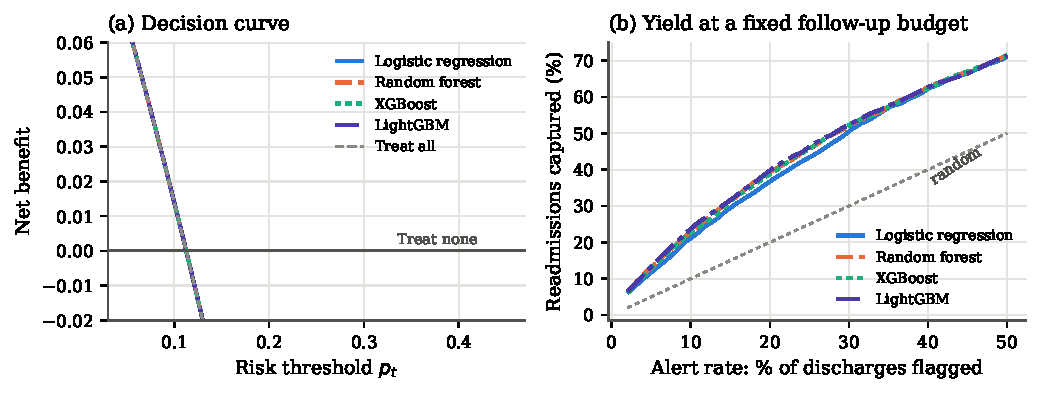
\includegraphics[width=\textwidth]{fig_utility.pdf}
\caption{(a) Decision curves: all models yield positive net benefit over treat-all and
treat-none across the plausible threshold range, and are mutually indistinguishable.
(b) Readmissions captured as a function of the alert budget.}
\label{fig:utility}
\end{figure}

\subsection{RQ2: the cost of encounter-level splitting}

\begin{table}[t]
\centering
\small
\caption{Optimism induced by encounter-level splitting. Model configurations are held fixed; only the split changes.}\label{tab:split}
\resizebox{\ifdim\width>\textwidth\textwidth\else\width\fi}{!}{\begin{tabular}{lcccccc}
\hline\noalign{\smallskip}
Model & AUROC (pat.) & AUROC (enc.) & $\Delta$ & AUPRC (pat.) & AUPRC (enc.) & $\Delta$ \\
\noalign{\smallskip}\hline\noalign{\smallskip}
Logistic regression & 0.664 & 0.665 & +0.0003 & 0.206 & 0.207 & +0.0013 \\
Random forest & 0.674 & 0.679 & +0.0043 & 0.219 & 0.223 & +0.0045 \\
XGBoost & 0.675 & 0.678 & +0.0028 & 0.217 & 0.219 & +0.0025 \\
LightGBM & 0.677 & 0.680 & +0.0034 & 0.223 & 0.222 & -0.0012 \\
\noalign{\smallskip}\hline
\end{tabular}
}
\\[3pt]
\begin{minipage}{\textwidth}\centering {\footnotesize \emph{pat.} = patient-disjoint split; \emph{enc.} = naive random split of encounters, in which 36\% of test patients also appear in training.}\end{minipage}
\end{table}


A naive stratified split of encounters places 35.8\% of test patients also in the
training set. The expectation --- ours included --- was that this would inflate
performance appreciably. It does not. Averaged over the four models the AUROC gain
from leaking is $+0.0027$, the largest relative AUPRC gain is $+2.1\%$ (random
forest), and for LightGBM the ``leaked'' estimate is marginally \emph{worse}
(Table~\ref{tab:split}, Fig.~\ref{fig:leakage}). We report this negative result
plainly because it revises a widely repeated methodological warning: on this
benchmark, patient overlap is real but its effect is an order of magnitude smaller
than the differences between published AUROC values, so existing encounter-level
results are not materially inflated by it.

The explanation is instructive. Leakage inflates performance when the model can
memorise something about a patient that it cannot infer from features. Here, what
makes a patient's admissions similar --- their history of utilisation --- is
\emph{already an explicit feature}. The model does not need to recognise the patient
because it can read the patient's history directly. Patient-level splitting remains
the correct default, since the guarantee costs nothing, but on this dataset it buys
rigour rather than a correction.

\begin{figure}[t]
\centering
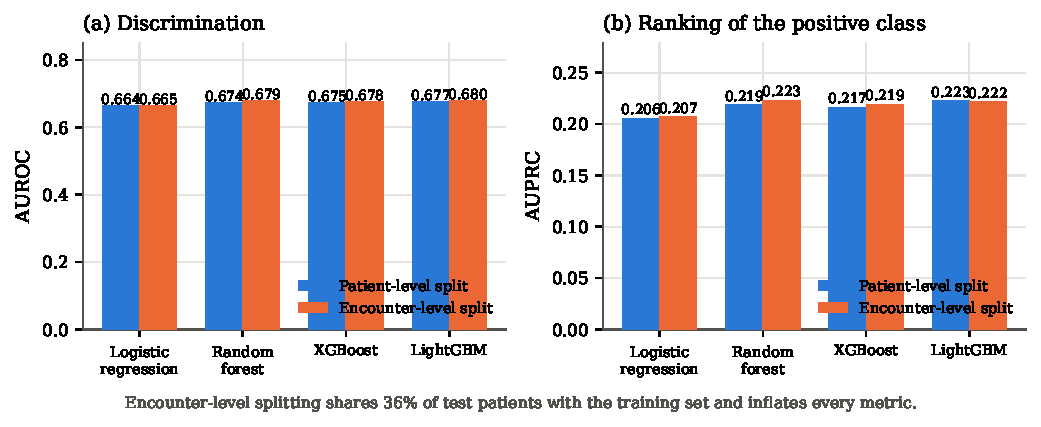
\includegraphics[width=\textwidth]{fig_leakage.pdf}
\caption{Patient-level versus encounter-level splitting. Despite 35.8\% patient
overlap, the optimism is negligible for every model family.}
\label{fig:leakage}
\end{figure}

\subsection{RQ3: imbalance corrections}

\begin{table}[t]
\centering
\small
\caption{Effect of class-imbalance treatments on a fixed LightGBM configuration.}\label{tab:imbalance}
\resizebox{\textwidth}{!}{\begin{tabular}{lcccccc}
\hline\noalign{\smallskip}
Imbalance treatment & AUROC & AUPRC & Brier & ECE & Mean $\hat p$ & Sens@10\% \\
\noalign{\smallskip}\hline\noalign{\smallskip}
None & 0.676 & 0.223 & 0.095 & 0.003 & 0.113 & 23.7 \\
Class weights & 0.677 & 0.223 & 0.220 & 0.343 & 0.456 & 23.5 \\
SMOTE (1:1) & 0.675 & 0.218 & 0.096 & 0.009 & 0.119 & 23.1 \\
SMOTE-NC (1:1) & 0.601 & 0.155 & 0.142 & 0.159 & 0.271 & 16.7 \\
Undersampling (1:1) & 0.672 & 0.214 & 0.226 & 0.351 & 0.464 & 22.5 \\
None + isotonic & 0.674 & 0.211 & 0.095 & 0.005 & 0.112 & 34.1 \\
\noalign{\smallskip}\hline
\end{tabular}
}
\\[3pt]
\begin{minipage}{\textwidth}\centering {\footnotesize Identical LightGBM configuration throughout; only the treatment of the class distribution changes. The observed event rate in the test set is 0.113.}\end{minipage}
\end{table}


Holding the LightGBM configuration fixed and varying only the treatment of the class
distribution produces the clearest result in this study
(Table~\ref{tab:imbalance}, Fig.~\ref{fig:imbalance}). No correction improves ranking:
the uncorrected model achieves the best AUPRC (0.223), and every correction is equal
or worse. All of them damage the probabilities. Class weighting and undersampling
raise the mean predicted risk from the observed 0.113 to 0.46, inflating ECE from
0.003 to above 0.34; the resulting scores are not risks in any usable sense, and a
clinician told that a patient's readmission probability is 46\% would be wrong by a
factor of four.

Two subtler observations deserve recording. First, plain SMOTE on the one-hot design
matrix is close to inert: after training on a perfectly balanced sample the mean
predicted risk remains at the natural prevalence. Interpolating between one-hot rows
produces \emph{fractional} category values that never occur in real records, so the
learner can separate synthetic from genuine minority cases and largely ignores them.
Second, SMOTE-NC, which respects the categorical structure and therefore actually
oversamples, is the worst performer of all: it reduces AUPRC to 0.155, a 30\% relative
loss. The apparent harmlessness of ordinary SMOTE in published work may in part be an
artefact of this encoding pathology rather than evidence that the method is benign.

Isotonic recalibration on a patient-disjoint calibration split restores calibration
(ECE 0.005) at a small AUPRC cost from binning, and is the route we recommend where
corrected models are already in use.

\begin{figure}[t]
\centering
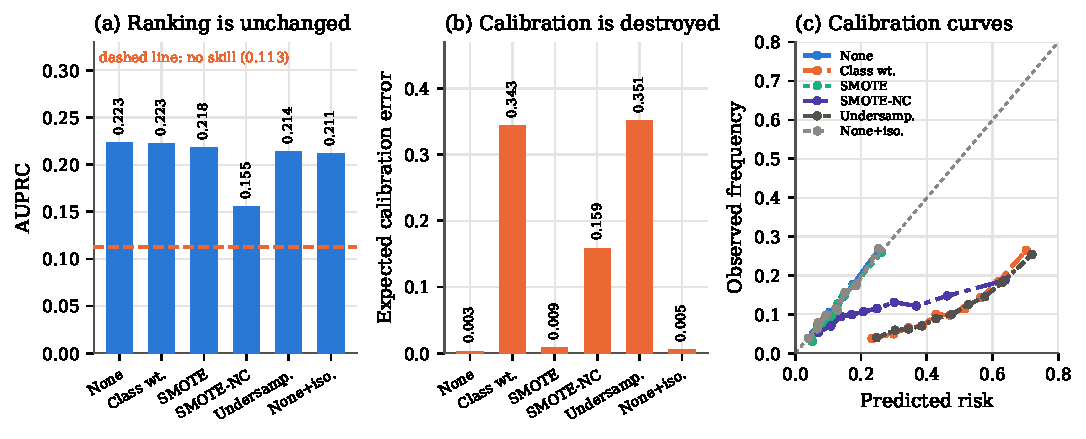
\includegraphics[width=\textwidth]{fig_imbalance.pdf}
\caption{Effect of imbalance treatments on the same LightGBM configuration. Ranking
(a) is flat; calibration (b, c) is destroyed by weighting and undersampling.}
\label{fig:imbalance}
\end{figure}

\subsection{RQ4: where the signal lives}
\label{sec:ablation}

\begin{table}[t]
\centering
\small
\caption{Feature-block ablation on the patient-disjoint test set.}\label{tab:ablation}
\resizebox{\ifdim\width>\textwidth\textwidth\else\width\fi}{!}{\begin{tabular}{lcccc}
\hline\noalign{\smallskip}
Feature set & $k$ & AUROC & AUPRC & $\Delta$AUPRC vs.\ full \\
\noalign{\smallskip}\hline\noalign{\smallskip}
+ Demographic & 3 & 0.510 & 0.117 & $-0.1066$ \\
+ Administrative & 8 & 0.605 & 0.167 & $-0.0561$ \\
+ Clinical & 22 & 0.625 & 0.172 & $-0.0508$ \\
+ Medication & 27 & 0.632 & 0.176 & $-0.0469$ \\
+ Prior utilisation & 34 & 0.676 & 0.223 & $+0.0000$ \\
- Demographic & 31 & 0.676 & 0.223 & $-0.0002$ \\
- Administrative & 29 & 0.652 & 0.208 & $-0.0153$ \\
- Clinical & 20 & 0.671 & 0.219 & $-0.0043$ \\
- Medication & 29 & 0.674 & 0.221 & $-0.0018$ \\
- Prior utilisation & 27 & 0.632 & 0.176 & $-0.0469$ \\
\noalign{\smallskip}\hline
\end{tabular}
}
\\[3pt]
\begin{minipage}{\textwidth}\centering {\footnotesize Upper block: blocks added cumulatively. Lower block: each block removed from the full model. Uncorrected LightGBM, patient-level split.}\end{minipage}
\end{table}


The ablation (Table~\ref{tab:ablation}, Fig.~\ref{fig:ablation}) is unambiguous.
Demographics alone are \emph{non-informative}: AUROC 0.510, AUPRC 0.117 against a
no-skill 0.113. Administrative variables --- chiefly discharge disposition, payer code
and admitting specialty --- lift AUROC to 0.605 with no clinical information
whatsoever. The 14 clinical variables add 0.005 AUPRC on top, and the medication block
a further 0.004. Prior utilisation then adds more than all other blocks combined,
taking AUPRC from 0.176 to 0.223. Leave-one-out confirms the ordering: removing prior
utilisation costs $-0.047$ AUPRC, administrative variables $-0.015$, clinical
$-0.004$, medication $-0.002$, and demographics $-0.0002$.

\begin{figure}[t]
\centering
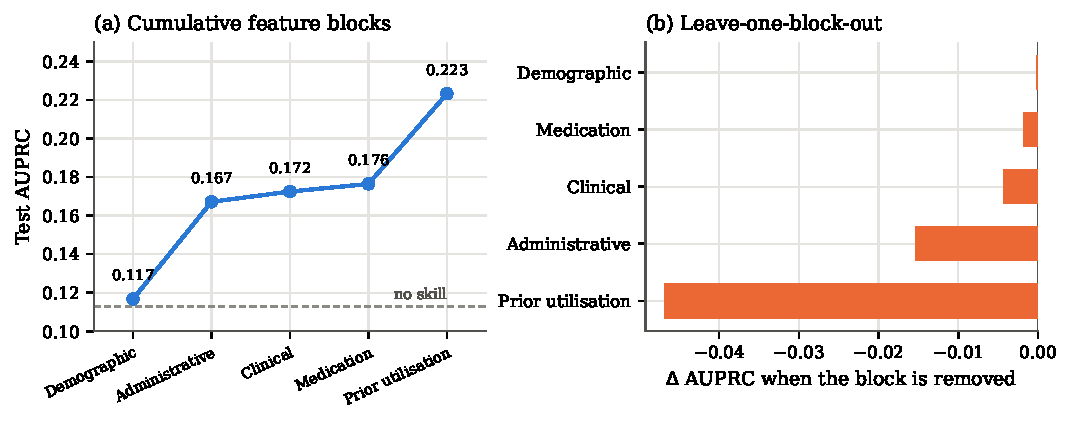
\includegraphics[width=\textwidth]{fig_ablation.pdf}
\caption{Feature-block ablation. Prior utilisation dominates; demographics contribute
nothing measurable.}
\label{fig:ablation}
\end{figure}

\subsection{Interpretability}

\begin{figure}[t]
\centering
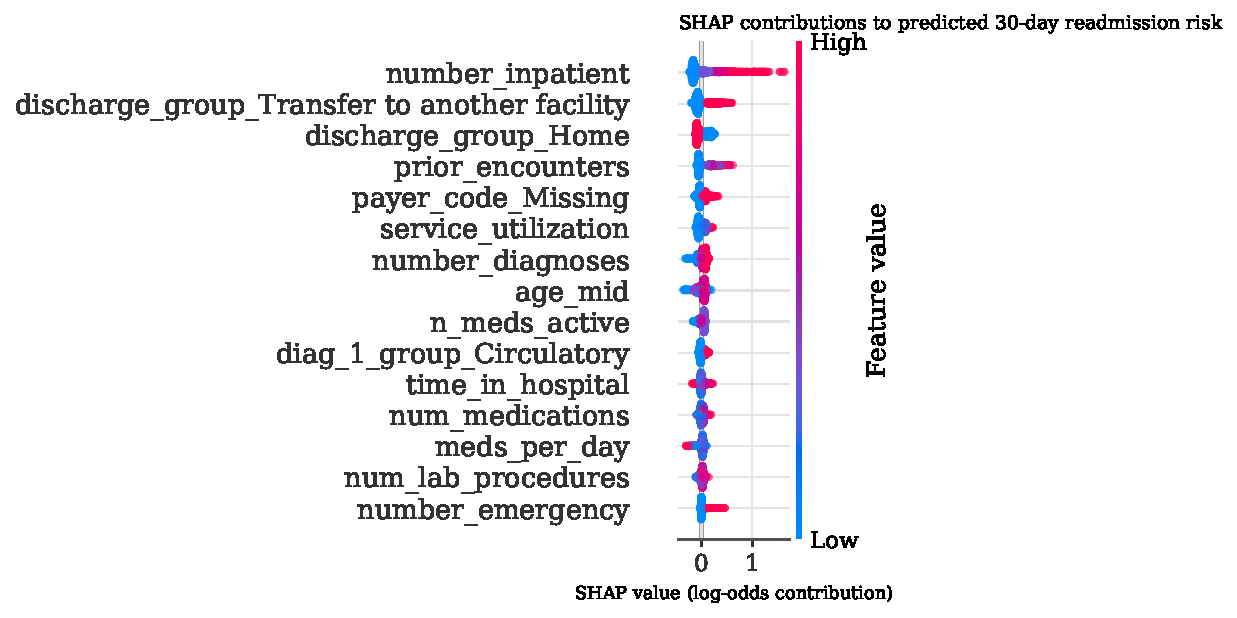
\includegraphics[width=0.85\textwidth]{fig_shap.pdf}
\caption{TreeSHAP attributions for the uncorrected LightGBM model on 3{,}000 test
encounters.}
\label{fig:shap}
\end{figure}

SHAP attributions~\cite{lundberg2017} for the uncorrected model and odds ratios from
the logistic regression agree closely (Table~\ref{tab:predictors}), which is
reassuring given how differently the two models are fitted. The number of prior
inpatient visits dominates both. Discharge to another facility raises the odds of
readmission by 38\% relative to the average encounter while discharge home lowers them
by 23\%; a missing payer code is associated with 19\% higher odds, and a nephrology
admitting specialty with 26\%. That non-clinical, administrative variables sit among
the strongest predictors is a finding about the system rather than the patient, and we
return to it below.

\begin{table}[t]
\centering
\small
\caption{Strongest predictors: logistic-regression odds ratios and SHAP ranking.}\label{tab:predictors}
\begin{tabular}{lcc}
\hline\noalign{\smallskip}
Predictor (encoded) & Odds ratio (LR) & SHAP rank \\
\noalign{\smallskip}\hline\noalign{\smallskip}
discharge: Transfer to another facility & 1.38 & 2 \\
discharge: Home & 0.77 & 3 \\
diagnosis 2: Neoplasms & 1.29 & -- \\
specialty: Nephrology & 1.26 & -- \\
specialty: Obstetrics \& Gynaecology & 0.81 & -- \\
diagnosis 3: Missing & 0.82 & -- \\
prior inpatient visits & 1.19 & 1 \\
payer: Missing & 1.19 & 5 \\
specialty: Cardiothoracic surgery & 0.84 & -- \\
specialty: Reconstructive orthopaedics & 0.85 & -- \\
payer: OG & 1.17 & -- \\
diagnosis 3: Neoplasms & 1.16 & -- \\
diagnosis 2: Respiratory & 0.87 & -- \\
diagnosis 1: Respiratory & 0.87 & -- \\
no diabetes medication & 0.88 & -- \\
\noalign{\smallskip}\hline
\end{tabular}

\\[3pt]
\begin{minipage}{\textwidth}\centering {\footnotesize Odds ratios from the $L_2$-regularised logistic regression (standardised numeric predictors); SHAP rank is the position in the mean $|$SHAP$|$ ordering of the LightGBM model (`--' = outside the top 15).}\end{minipage}
\end{table}


\section{Discussion}

\paragraph{Relation to existing work.} Our AUROC of 0.677 sits squarely on the median
of 0.68 that Mahmoudi et al.~\cite{mahmoudi2020} report across 41 EHR-based readmission
models, and in the same band as Kansagara et al.'s~\cite{kansagara2011} earlier
survey, despite two decades of methodological progress between them. On this benchmark
specifically, Liu et al.~\cite{liu2024} likewise found tree ensembles ahead of a deep
LSTM, and Shang et al.~\cite{shang2021} likewise found random forests competitive; our
ranking (LightGBM $\approx$ random forest $>$ XGBoost $>$ logistic regression)
reproduces theirs while adding the observation that the gap over logistic regression,
although statistically reliable, is 0.017 AUPRC --- well below what would change a
discharge decision. The persistent finding across the literature and this study is a
\emph{data} ceiling, not a modelling one: the determinants of readmission that matter
most, such as social support, medication adherence, housing and outpatient
follow-up, are simply not recorded in these tables.

Our imbalance results agree closely with van den Goorbergh et al.~\cite{goorbergh2022}
and Welvaars et al.~\cite{welvaars2023}, extending both from logistic regression and
from a single-centre urology cohort to gradient boosting on a public benchmark, and
adding the encoding-pathology observation about SMOTE that, to our knowledge, has not
been reported for this dataset. Given that Lu and Uddin~\cite{lu2022} and many others
undersample as a preprocessing step on exactly these data, the implication is
practical: their reported probabilities should not be read as risks.

Our leakage result cuts the other way and is worth stating against our own prior.
Following Kapoor and Narayanan~\cite{kapoor2023} we expected encounter-level splitting
to be a material source of optimism; measured, it is not. Methodological warnings
deserve empirical calibration as much as models do.

\paragraph{Implications.} For practice, a 10\% alert rate capturing 23.5\% of
readmissions at 26.5\% precision is usable --- it roughly doubles the yield of
untargeted follow-up --- but only if the score is calibrated, which rules out the
imbalance corrections that dominate published pipelines. For research, the ablation
suggests the productive direction is not another architecture but linkage to the data
that is missing: outpatient follow-up, social determinants and medication adherence.
For governance, the prominence of payer code and admitting specialty is a warning:
a model may be learning how the health system treats different patients rather than
how sick they are, and deploying it could entrench that pattern.

\paragraph{Limitations.} (i) The data are from 1999--2008 and predate the HRRP;
absolute rates and practice patterns have shifted, so external validity to current
care is limited. (ii) Readmissions to a different hospital system are invisible, so
the outcome is under-ascertained and our prevalence is a lower bound. (iii) The
feature \texttt{prior\_encounters} is defined within the observation window and would
require a fixed lookback in deployment. (iv) We tuned under a modest randomised-search
budget on three folds; a larger budget might shift model ordering slightly, though the
narrow spread makes a reversal of the substantive conclusion unlikely. (v) Fairness
was not formally audited: we report that race is non-informative for prediction here,
but a full subgroup analysis of error rates is future work. (vi) The single
train/test split, though patient-disjoint and large, gives one realisation; repeated
splits would tighten the interval estimates.

\section{Conclusion}

Under a strictly patient-level protocol on 99{,}340 encounters, gradient boosting
predicts 30-day readmission with AUROC 0.677 and AUPRC 0.223, a small but reliable
margin over regularised logistic regression. Three methodological conclusions follow
from the experiments rather than from convention. Encounter-level splitting, although
it shares 36\% of test patients with training, inflates performance negligibly on this
benchmark --- a negative result we report because the opposite is widely assumed.
Imbalance corrections improve nothing and destroy calibration, with categorical-aware
SMOTE-NC losing 30\% of AUPRC outright. And the predictive signal is overwhelmingly
historical and administrative rather than clinical or demographic: demographics alone
give AUROC 0.510, while prior utilisation alone accounts for more than all other
feature blocks combined. The ceiling on this task is set by what hospital records do
not contain, and the useful next step is better data rather than better classifiers.

\paragraph{Reproducibility.} Data source, analysis notebook, generated figures and
tables, the literature search log and the complete prompt history accompany this
submission; all results derive from a single deterministic run with fixed seeds.

\bibliographystyle{splncs04}
\bibliography{refs}

\appendix
\section{Screening record}
\label{app:screening}
\setlength{\tabcolsep}{4pt}
\begin{longtable}{rp{4.9cm}p{1.35cm}p{4.6cm}}
\caption{Screening record for all 77 de-duplicated candidates. Reason codes: R~=~review or commentary without a primary model, O~=~outcome outside the readmission construct, D~=~data modality outside structured tabular records, M~=~no predictive performance reported, Y~=~published before 2015.}\label{tab:screening}\\
\toprule \# & Title & Decision & Reason \\ \midrule
\endfirsthead
\toprule \# & Title & Decision & Reason \\ \midrule
\endhead
\bottomrule
\endfoot
0 & Deep learning for healthcare: review, opportunities and challenges & exclude & R: narrative review, no readmission model \\
1 & Scalable and accurate deep learning with electronic health records & include & 30-day readmission among predicted endpoints, structured EHR \\
2 & MIMIC-IV, a freely accessible electronic health record dataset & exclude & R: data resource descriptor, no prediction model \\
3 & Machine Learning-Based Prediction of Heart Failure Readmission or Death & include & 30-day HF readmission, tabular linked data, imbalance addressed \\
4 & Application of machine learning in predicting hospital readmissions: a scop... & exclude & R: scoping review; retained as background evidence \\
5 & Machine Learning and Data Mining Methods in Diabetes Research & exclude & R: review of diabetes ML broadly, not readmission \\
6 & ClinicalBERT: Modeling Clinical Notes and Predicting Hospital Readmission & exclude & D: prediction from free-text notes, not structured tabular records \\
7 & Next-generation phenotyping of electronic health records & exclude & R: perspective on EHR data quality, no model \\
8 & Use of electronic medical records in development and validation of risk pre... & exclude & R: systematic review; retained as background evidence \\
9 & Opportunities and challenges in developing deep learning models using EHR data & exclude & R: systematic review of architectures \\
10 & Key challenges for delivering clinical impact with artificial intelligence & exclude & R: commentary on AI translation \\
11 & Readmission prediction using deep learning on electronic health records & include & 30-day CHF readmission, cost-sensitive LSTM on EHR \\
12 & The effects of data sources, cohort selection, and outcome definition & exclude & Y: published 2014; retained as background on design choices \\
13 & Revolutionizing healthcare: the role of artificial intelligence in clinical... & exclude & R: educational review \\
14 & Federated Learning for Healthcare Informatics & exclude & O: federated learning survey, outcome not readmission \\
15 & BEHRT: Transformer for Electronic Health Records & exclude & O: predicts 301 future diagnoses, not readmission \\
16 & Effect of Aliskiren on Postdischarge Mortality and Heart Failure Readmissions & exclude & O: randomised drug trial, not a prediction model \\
17 & Survey on deep learning with class imbalance & exclude & R: methodological survey; retained as background on imbalance \\
18 & Machine learning prediction in cardiovascular diseases: a meta-analysis & exclude & O: diagnosis of CVD, not readmission \\
19 & Explainable Artificial Intelligence (XAI): Concepts, taxonomies, opportunities & exclude & R: XAI survey, non-clinical \\
20 & Multimodal machine learning in precision health: A scoping review & exclude & R: scoping review of data fusion \\
21 & Analysis and prediction of unplanned ICU readmission using RNN-LSTM & include & unplanned ICU readmission from MIMIC-III structured data \\
22 & Emergency department triage prediction of clinical outcomes & exclude & O: triage acuity/critical outcomes, not readmission \\
23 & Predictors of 30-Day Unplanned Readmission After Carotid Artery Stenting & include & 30-day readmission, Nationwide Readmission Database, ML comparison \\
24 & Machine learning for clinical decision support in infectious diseases & exclude & O: infection diagnosis/management \\
25 & Patient clustering improves efficiency of federated machine learning & exclude & O: outcomes are mortality and length of stay \\
26 & Combining structured and unstructured data for predictive models & exclude & D: fusion with clinical notes; outcome not 30-day readmission \\
27 & Machine Learning-Enabled 30-Day Readmission Model for Stroke Patients & include & 30-day readmission after ischaemic stroke, EHR, 5 algorithms \\
28 & Secure and robust machine learning for healthcare: A survey & exclude & R: security/privacy survey \\
29 & Mining Electronic Health Records (EHRs) & exclude & R: methods survey \\
30 & Nutritional assessment: comparison of clinical assessment and objective var... & exclude & M: association study, no discrimination metrics reported \\
31 & Moving beyond regression techniques in cardiovascular risk prediction & exclude & O: mortality after myocardial infarction \\
32 & A machine learning model to predict the risk of 30-day readmissions in hear... & include & 30-day HF readmission from longitudinal EMR, utilisation features \\
33 & Neural networks versus Logistic regression for 30 days all-cause readmission & include & 30-day all-cause readmission, claims data, NN vs LR comparison \\
34 & Significance of machine learning in healthcare: Features, pillars and appli... & exclude & R: general overview \\
35 & Prediction of 30-Day All-Cause Readmissions in Patients Hospitalized for He... & include & 30-day readmission, ML vs conventional logistic models \\
36 & Predicting Hospital Readmission among Diabetics using Deep Learning & include & same benchmark dataset, CNN + feature engineering \\
37 & Impact of HbA1c Measurement on Hospital Readmission Rates & exclude & Y: 2014; retained as the provenance record of the dataset used here \\
38 & Challenges and opportunities beyond structured data in analysis of EHR & exclude & R: review of unstructured-data analytics \\
39 & Assessment of Machine Learning vs Standard Prediction Rules for Readmissions & include & 30-day readmission, ML rank score vs LACE/HOSPITAL rules \\
40 & A stacking-based model for predicting 30-day all-cause readmissions in AMI & include & 30-day readmission, stacking ensemble, undersampling (NCR) \\
41 & Machine Learning for Clinical Outcome Prediction & exclude & R: review of outcome-prediction methodology \\
42 & Machine Learning for Healthcare: On the Verge of a Major Shift & exclude & R: introductory review \\
43 & Deep learning for electronic health records: a comparative review & exclude & R: comparative review of architectures \\
44 & Comparison of machine learning models for predicting 30-day readmission (di... & include & same benchmark dataset, 10 ML + 1 DL model comparison \\
45 & Opportunities and challenges in developing risk prediction models with EHR ... & exclude & R: systematic review of EHR modelling practice \\
46 & Current Challenges and Future Opportunities for XAI in ML-Based CDSS & exclude & R: XAI systematic review \\
47 & Deep representation learning of patient data from EHR: a systematic review & exclude & R: systematic review \\
48 & A new analytical framework for missing data imputation and classification & include & HF readmission with explicit missing-data framework (GPLVM) \\
49 & Predicting healthcare trajectories from medical records (DeepCare) & include & unplanned readmission for diabetes cohorts from EHR sequences \\
50 & The 30-days hospital readmission risk in diabetic patients & include & same benchmark dataset, RF / NB / decision-tree ensemble \\
51 & Multitask learning and benchmarking with clinical time series data & exclude & O: mortality, length of stay, phenotyping benchmarks \\
52 & Predicting Unplanned Readmissions Following a Hip or Knee Arthroplasty & include & 30-day readmission after arthroplasty; structured + note features \\
53 & Interpretability of machine learning-based prediction models in healthcare & exclude & R: interpretability review \\
54 & A survey on datasets for fairness-aware machine learning & exclude & O: fairness benchmark survey \\
55 & Imbalanced class distribution and performance evaluation metrics & exclude & R: systematic review; retained as background on metric choice \\
56 & Med-BERT: pretrained contextualized embeddings on structured EHR & exclude & O: disease-onset prediction, not readmission \\
57 & Comparison of Conventional Statistical Methods with Machine Learning in Med... & exclude & R: methodological comparison review \\
58 & Deep representation learning of EHR to unlock patient stratification & exclude & O: unsupervised stratification, no readmission outcome \\
59 & Explainable Stacking-Based Model for Predicting Hospital Readmission for Di... & include & same benchmark dataset, stacking + RUS + explainability \\
60 & Shifting machine learning for healthcare from development to deployment & exclude & R: perspective on deployment \\
61 & Applying Artificial Intelligence to Wearable Sensor Data & exclude & D: wearable sensor data, not inpatient records \\
62 & Predictive Modeling of the Hospital Readmission Risk from Claims Data (COPD) & include & 30-day COPD readmission, 111,992 patients, deep and non-deep models \\
63 & Nationwide hospital admission data statistics and disease-specific readmission & include & disease-specific 30-day readmission on national admission data \\
64 & Artificial intelligence and machine learning in precision and genomic medicine & exclude & D: genomics; also retracted \\
65 & An explainable machine learning framework for lung cancer LOS prediction & exclude & O: length of stay; retained as background on resampling effects \\
66 & Early prediction of ICU readmissions using classification algorithms & include & ICU readmission, tabular clinical predictors, classifier comparison \\
67 & Machine learning based prediction models for cardiovascular disease risk & exclude & O: 5-10 year CVD risk, not readmission \\
68 & Toward Predicting 30-Day Readmission Among Oncology Patients & include & 30-day readmission, patient/provider/community features, LightGBM \\
69 & Explainable, trustworthy, and ethical machine learning for healthcare & exclude & R: survey of explainability and ethics \\
70 & Data Mining in Healthcare - A Review & exclude & R: review of data-mining applications \\
71 & Reducing patient mortality, LOS and readmissions through sepsis prediction & exclude & O: sepsis onset prediction; readmission only a downstream QI metric \\
72 & Machine Learning-Based Early Prediction of Sepsis Using EHR & exclude & O: sepsis onset \\
73 & On the interpretability of machine learning-based model for predicting hype... & exclude & O: hypertension risk \\
74 & Leveraging Machine Learning Techniques to Forecast Patient Prognosis After PCI & exclude & O: prognosis/mortality after PCI \\
75 & Association of Surgical and Hospital Volume with 30-Day Readmission Rates & exclude & M: association analysis, no predictive performance reported \\
76 & Implications of resampling data to address the class imbalance problem (IRCIP) & include & 30-day readmission case study; resampling vs calibration - core to RQ3 \\
\end{longtable}
\setlength{\tabcolsep}{6pt}

\end{document}
